\documentclass[11pt]{article}

\usepackage[top=0.5in, bottom=0.5in, left=0.5in, right=0.5in]{geometry}
\usepackage{authblk}
\usepackage{hyperref}
\usepackage[utf8]{inputenc}
\usepackage{amsmath}
\usepackage{amsfonts}
\usepackage{amssymb}
\usepackage{siunitx}
\usepackage{graphicx}
\usepackage{subcaption}
\usepackage{float}
\usepackage[nottoc,numbib]{tocbibind}
\usepackage{biblatex}

\bibliography{references.bib}

\newcommand{\email}[1]{\texttt{\href{mailto:#1}{#1}}}

\title{CMSC 478 Project Milestone}
\author{Robert Rose}

\makeatletter
\let\inserttitle\@title
\let\insertauthor\@author
\makeatother

\begin{document}

\begin{center}
  \LARGE{\inserttitle}

  \Large{\insertauthor}
\end{center}

\section{Getting Data}

My project is based off of a currently running Kaggle competition and as a result, the data can be
found on the Kaggle website.\cite{competition} Additionally, the Python notebook with my work can
be found pre-rendered as a Kaggle Kernel, which is what I recommend using since it takes quite some
time to run all the way through.\cite{clustering}

\section{Work So Far}

So far I've worked on the clustering approach using various clustering methods and Principal Component
Analysis.\cite{clustering} Additionally, I computed some basic linear regression models to test 
various features extracted from the clusters. The linear regression models were based on a Kernel by 
another Kaggler which was pretty well organized so I've used it as a reference for several parts 
of my project, including the test-train split in addition to the baseline features used in the 
linear model.\cite{feature-engineering}

Although in my proposal I planned on using $K$-fold cross validation, I felt that using a split on the
match ids, as suggested in another Kernel, was a better way to split.\cite{feature-engineering}
Since the prediction target is players, but the data is separated into matches that have non-independent
variables (e.g. the winPlacePerc for one player in a match is determined by how well they did compared to
other players in the match), a split on matchId makes the most sense so we can gather the most relevant
information.

\section{Results}

The current result is a fairly promising results on a simple linear model. Since we are splitting the
data into a test and validation set, albeit not cross validation, a lower error rate typically suggests
a more effective model. As you can see in Table 1, adding my own features using clusters did result in a 
lower error rate, suggesting there is some signal in the features I generated. Table 1 contains the 
centroid and cluster features for several N number of clusters as well as the original data without 
any added features. Included is mean absolute error on the validation set as "Score" and the amount 
of time it took to execute under "Execution Time".

\begin{table}[h]
 \centering
 \caption{Cluster and Centroid Simple Model Results}
 \begin{tabular}{||c c c c||} 
 \hline
 Index & Name & Score & Execution Time \\ [0.5ex] 
 \hline\hline
 4 & kmeans\_4\_centroids & 0.089267 &	47.68s \\ 
 \hline
 5 & kmeans\_5\_clusters & 0.089349 & 47.73s \\
 \hline
 1 & kmeans\_3\_clusters & 0.089359 &	46.66s \\
 \hline
 6 & kmeans\_5\_centroids & 0.089408 &	48.28s \\
 \hline
 3 & kmeans\_4\_clusters & 0.089562 & 48.72s \\
 \hline
 2 & kmeans\_3\_centroids & 0.089677 & 47.29s \\
 \hline
 0 & original &	0.092813 & 28.97s \\ 
 \hline
\end{tabular}
\end{table}

The \textbf{clusters} features are a series of one-hot encoded features as to which of the N clusters the data point 
fell in. The \textbf{centroid} features are a series of features computed by taking the euclidean distance to each of 
the N clusters. Each experiment in the linear model is actually N number of features, where N is the number of clusters.
I tried the linear experiments with 4-cluster $K$-means, 5-cluster $K$-means and 3-cluster $K$-means as those seemed 
to be the most logically arranged clusters. Figure 1 is the first 100,000 2-component PCA points with 5-cluster K-means
applied.

\begin{figure}[h]
\caption{K-Means with Five Clusters}
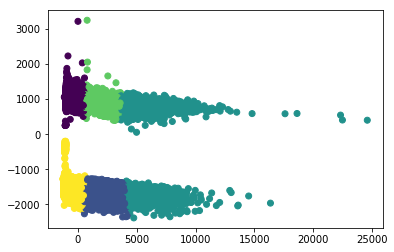
\includegraphics[width=0.6\textwidth]{clusters.png}
\centering
\end{figure}

The 2-component PCA explained 74.9\% of the total variance in the dataset. Although the rule of thumb is typically 80\% of
variance explained, adding one additional PCA component brought the explained variance to 96.1\%, which I felt was too high
to be trusted. Additionally, keeping only two dimensions meant that I could easily plot and cluster the data.

\section{Next Steps}

My next steps will likely include stepping away from subjects we've discussed in class to explore tree based methods such as
LightGBM or XGBoost in order to take the features I've engineered using PCA and $K$-means to produce predictions for the competition.
I hope that all the work I've done creating clustering features is not for naught and that more advanced models use them 
successfully.

Additionally, I need to explore the scikit-learn documentation to see if there is a way to split the data using $K$-fold cross
validation using the matchIds as the key to split. I don't know if this is possible currently in sklearn, if it's not I will
likely need to hand write the $K$-fold cross validation.

\printbibliography

\end{document}
